
%% bare_conf.tex
%% V1.3
%% 2007/01/11
%% by Michael Shell
%% See:
%% http://www.michaelshell.org/
%% for current contact information.
%%
%% This is a skeleton file demonstrating the use of IEEEtran.cls
%% (requires IEEEtran.cls version 1.7 or later) with an IEEE conference paper.
%%
%% Support sites:
%% http://www.michaelshell.org/tex/ieeetran/
%% http://www.ctan.org/tex-archive/macros/latex/contrib/IEEEtran/
%% and
%% http://www.ieee.org/

%%*************************************************************************
%% Legal Notice:
%% This code is offered as-is without any warranty either expressed or
%% implied; without even the implied warranty of MERCHANTABILITY or
%% FITNESS FOR A PARTICULAR PURPOSE! 
%% User assumes all risk.
%% In no event shall IEEE or any contributor to this code be liable for
%% any damages or losses, including, but not limited to, incidental,
%% consequential, or any other damages, resulting from the use or misuse
%% of any information contained here.
%%
%% All comments are the opinions of their respective authors and are not
%% necessarily endorsed by the IEEE.
%%
%% This work is distributed under the LaTeX Project Public License (LPPL)
%% ( http://www.latex-project.org/ ) version 1.3, and may be freely used,
%% distributed and modified. A copy of the LPPL, version 1.3, is included
%% in the base LaTeX documentation of all distributions of LaTeX released
%% 2003/12/01 or later.
%% Retain all contribution notices and credits.
%% ** Modified files should be clearly indicated as such, including  **
%% ** renaming them and changing author support contact information. **
%%
%% File list of work: IEEEtran.cls, IEEEtran_HOWTO.pdf, bare_adv.tex,
%%                    bare_conf.tex, bare_jrnl.tex, bare_jrnl_compsoc.tex
%%*************************************************************************

% *** Authors should verify (and, if needed, correct) their LaTeX system  ***
% *** with the testflow diagnostic prior to trusting their LaTeX platform ***
% *** with production work. IEEE's font choices can trigger bugs that do  ***
% *** not appear when using other class files.                            ***
% The testflow support page is at:
% http://www.michaelshell.org/tex/testflow/



% Note that the a4paper option is mainly intended so that authors in
% countries using A4 can easily print to A4 and see how their papers will
% look in print - the typesetting of the document will not typically be
% affected with changes in paper size (but the bottom and side margins will).
% Use the testflow package mentioned above to verify correct handling of
% both paper sizes by the user's LaTeX system.
%
% Also note that the "draftcls" or "draftclsnofoot", not "draft", option
% should be used if it is desired that the figures are to be displayed in
% draft mode.
%
\documentclass[conference]{IEEEtran}
% Add the compsoc option for Computer Society conferences.
%
% If IEEEtran.cls has not been installed into the LaTeX system files,
% manually specify the path to it like:
% \documentclass[conference]{../sty/IEEEtran}



\usepackage[english]{babel}
%\usepackage[english,thai]{babel}
%\selectlanguage{english}
\usepackage[utf8x]{inputenc}
\usepackage{fonts-tlwg}




\usepackage{amsfonts,mathrsfs}
\usepackage{amsthm, amsmath}
\usepackage{enumerate}
\usepackage{color}
\usepackage{graphicx}
\usepackage{verbatim}
\usepackage{placeins}
\usepackage{caption}
\usepackage{everysel}
\usepackage{keyval}
\usepackage{ragged2e}
\usepackage{subfig}
\usepackage{float}

\newcommand{\norm}[1]{|| #1 || } 
\definecolor{airforceblue}{rgb}{0.36, 0.54, 0.66}
\definecolor{awesome}{rgb}{1.0, 0.13, 0.32}
\newcommand{\col}[1]{\textcolor{awesome}{#1}}
\newcommand{\Tone}{\Theta^{(1)}}
\newcommand{\Ttwo}{\Theta^{(2)}}


\usepackage{tikz}


%%% For Unicode
%\usepackage[utf8]{inputenc}
%\DeclareUnicodeCharacter{2014}{\dash}
%\DeclareRobustCommand\dash{%
%  \unskip\nobreak\thinspace\textemdash\allowbreak\thinspace\ignorespaces}
%\usepackage{CJKutf8} 
%\usepackage{ucs} 
%\usepackage[encapsulated]{CJK} 
%\newcommand{\myfont}{bsmi} % or {stheiti}, etc 

%\usepackage[utf8]{inputenc}
%\usepackage[T1]{fontenc}




% Some very useful LaTeX packages include:
% (uncomment the ones you want to load)


% *** MISC UTILITY PACKAGES ***
%
%\usepackage{ifpdf}
% Heiko Oberdiek's ifpdf.sty is very useful if you need conditional
% compilation based on whether the output is pdf or dvi.
% usage:
% \ifpdf
%   % pdf code
% \else
%   % dvi code
% \fi
% The latest version of ifpdf.sty can be obtained from:
% http://www.ctan.org/tex-archive/macros/latex/contrib/oberdiek/
% Also, note that IEEEtran.cls V1.7 and later provides a builtin
% \ifCLASSINFOpdf conditional that works the same way.
% When switching from latex to pdflatex and vice-versa, the compiler may
% have to be run twice to clear warning/error messages.






% *** CITATION PACKAGES ***
%
%\usepackage{cite}
% cite.sty was written by Donald Arseneau
% V1.6 and later of IEEEtran pre-defines the format of the cite.sty package
% \cite{} output to follow that of IEEE. Loading the cite package will
% result in citation numbers being automatically sorted and properly
% "compressed/ranged". e.g., [1], [9], [2], [7], [5], [6] without using
% cite.sty will become [1], [2], [5]--[7], [9] using cite.sty. cite.sty's
% \cite will automatically add leading space, if needed. Use cite.sty's
% noadjust option (cite.sty V3.8 and later) if you want to turn this off.
% cite.sty is already installed on most LaTeX systems. Be sure and use
% version 4.0 (2003-05-27) and later if using hyperref.sty. cite.sty does
% not currently provide for hyperlinked citations.
% The latest version can be obtained at:
% http://www.ctan.org/tex-archive/macros/latex/contrib/cite/
% The documentation is contained in the cite.sty file itself.






% *** GRAPHICS RELATED PACKAGES ***
%
\ifCLASSINFOpdf
  % \usepackage[pdftex]{graphicx}
  % declare the path(s) where your graphic files are
  % \graphicspath{{../pdf/}{../jpeg/}}
  % and their extensions so you won't have to specify these with
  % every instance of \includegraphics
  % \DeclareGraphicsExtensions{.pdf,.jpeg,.png}
\else
  % or other class option (dvipsone, dvipdf, if not using dvips). graphicx
  % will default to the driver specified in the system graphics.cfg if no
  % driver is specified.
  % \usepackage[dvips]{graphicx}
  % declare the path(s) where your graphic files are
  % \graphicspath{{../eps/}}
  % and their extensions so you won't have to specify these with
  % every instance of \includegraphics
  % \DeclareGraphicsExtensions{.eps}
\fi
% graphicx was written by David Carlisle and Sebastian Rahtz. It is
% required if you want graphics, photos, etc. graphicx.sty is already
% installed on most LaTeX systems. The latest version and documentation can
% be obtained at: 
% http://www.ctan.org/tex-archive/macros/latex/required/graphics/
% Another good source of documentation is "Using Imported Graphics in
% LaTeX2e" by Keith Reckdahl which can be found as epslatex.ps or
% epslatex.pdf at: http://www.ctan.org/tex-archive/info/
%
% latex, and pdflatex in dvi mode, support graphics in encapsulated
% postscript (.eps) format. pdflatex in pdf mode supports graphics
% in .pdf, .jpeg, .png and .mps (metapost) formats. Users should ensure
% that all non-photo figures use a vector format (.eps, .pdf, .mps) and
% not a bitmapped formats (.jpeg, .png). IEEE frowns on bitmapped formats
% which can result in "jaggedy"/blurry rendering of lines and letters as
% well as large increases in file sizes.
%
% You can find documentation about the pdfTeX application at:
% http://www.tug.org/applications/pdftex





% *** MATH PACKAGES ***
%
%\usepackage[cmex10]{amsmath}
% A popular package from the American Mathematical Society that provides
% many useful and powerful commands for dealing with mathematics. If using
% it, be sure to load this package with the cmex10 option to ensure that
% only type 1 fonts will utilized at all point sizes. Without this option,
% it is possible that some math symbols, particularly those within
% footnotes, will be rendered in bitmap form which will result in a
% document that can not be IEEE Xplore compliant!
%
% Also, note that the amsmath package sets \interdisplaylinepenalty to 10000
% thus preventing page breaks from occurring within multiline equations. Use:
%\interdisplaylinepenalty=2500
% after loading amsmath to restore such page breaks as IEEEtran.cls normally
% does. amsmath.sty is already installed on most LaTeX systems. The latest
% version and documentation can be obtained at:
% http://www.ctan.org/tex-archive/macros/latex/required/amslatex/math/





% *** SPECIALIZED LIST PACKAGES ***
%
%\usepackage{algorithmic}
% algorithmic.sty was written by Peter Williams and Rogerio Brito.
% This package provides an algorithmic environment fo describing algorithms.
% You can use the algorithmic environment in-text or within a figure
% environment to provide for a floating algorithm. Do NOT use the algorithm
% floating environment provided by algorithm.sty (by the same authors) or
% algorithm2e.sty (by Christophe Fiorio) as IEEE does not use dedicated
% algorithm float types and packages that provide these will not provide
% correct IEEE style captions. The latest version and documentation of
% algorithmic.sty can be obtained at:
% http://www.ctan.org/tex-archive/macros/latex/contrib/algorithms/
% There is also a support site at:
% http://algorithms.berlios.de/index.html
% Also of interest may be the (relatively newer and more customizable)
% algorithmicx.sty package by Szasz Janos:
% http://www.ctan.org/tex-archive/macros/latex/contrib/algorithmicx/




% *** ALIGNMENT PACKAGES ***
%
%\usepackage{array}
% Frank Mittelbach's and David Carlisle's array.sty patches and improves
% the standard LaTeX2e array and tabular environments to provide better
% appearance and additional user controls. As the default LaTeX2e table
% generation code is lacking to the point of almost being broken with
% respect to the quality of the end results, all users are strongly
% advised to use an enhanced (at the very least that provided by array.sty)
% set of table tools. array.sty is already installed on most systems. The
% latest version and documentation can be obtained at:
% http://www.ctan.org/tex-archive/macros/latex/required/tools/


%\usepackage{mdwmath}
%\usepackage{mdwtab}
% Also highly recommended is Mark Wooding's extremely powerful MDW tools,
% especially mdwmath.sty and mdwtab.sty which are used to format equations
% and tables, respectively. The MDWtools set is already installed on most
% LaTeX systems. The lastest version and documentation is available at:
% http://www.ctan.org/tex-archive/macros/latex/contrib/mdwtools/


% IEEEtran contains the IEEEeqnarray family of commands that can be used to
% generate multiline equations as well as matrices, tables, etc., of high
% quality.


%\usepackage{eqparbox}
% Also of notable interest is Scott Pakin's eqparbox package for creating
% (automatically sized) equal width boxes - aka "natural width parboxes".
% Available at:
% http://www.ctan.org/tex-archive/macros/latex/contrib/eqparbox/





% *** SUBFIGURE PACKAGES ***
%\usepackage[tight,footnotesize]{subfigure}
% subfigure.sty was written by Steven Douglas Cochran. This package makes it
% easy to put subfigures in your figures. e.g., "Figure 1a and 1b". For IEEE
% work, it is a good idea to load it with the tight package option to reduce
% the amount of white space around the subfigures. subfigure.sty is already
% installed on most LaTeX systems. The latest version and documentation can
% be obtained at:
% http://www.ctan.org/tex-archive/obsolete/macros/latex/contrib/subfigure/
% subfigure.sty has been superceeded by subfig.sty.



%\usepackage[caption=false]{caption}
%\usepackage[font=footnotesize]{subfig}
% subfig.sty, also written by Steven Douglas Cochran, is the modern
% replacement for subfigure.sty. However, subfig.sty requires and
% automatically loads Axel Sommerfeldt's caption.sty which will override
% IEEEtran.cls handling of captions and this will result in nonIEEE style
% figure/table captions. To prevent this problem, be sure and preload
% caption.sty with its "caption=false" package option. This is will preserve
% IEEEtran.cls handing of captions. Version 1.3 (2005/06/28) and later 
% (recommended due to many improvements over 1.2) of subfig.sty supports
% the caption=false option directly:
%\usepackage[caption=false,font=footnotesize]{subfig}
%
% The latest version and documentation can be obtained at:
% http://www.ctan.org/tex-archive/macros/latex/contrib/subfig/
% The latest version and documentation of caption.sty can be obtained at:
% http://www.ctan.org/tex-archive/macros/latex/contrib/caption/




% *** FLOAT PACKAGES ***
%
%\usepackage{fixltx2e}
% fixltx2e, the successor to the earlier fix2col.sty, was written by
% Frank Mittelbach and David Carlisle. This package corrects a few problems
% in the LaTeX2e kernel, the most notable of which is that in current
% LaTeX2e releases, the ordering of single and double column floats is not
% guaranteed to be preserved. Thus, an unpatched LaTeX2e can allow a
% single column figure to be placed prior to an earlier double column
% figure. The latest version and documentation can be found at:
% http://www.ctan.org/tex-archive/macros/latex/base/



%\usepackage{stfloats}
% stfloats.sty was written by Sigitas Tolusis. This package gives LaTeX2e
% the ability to do double column floats at the bottom of the page as well
% as the top. (e.g., "\begin{figure*}[!b]" is not normally possible in
% LaTeX2e). It also provides a command:
%\fnbelowfloat
% to enable the placement of footnotes below bottom floats (the standard
% LaTeX2e kernel puts them above bottom floats). This is an invasive package
% which rewrites many portions of the LaTeX2e float routines. It may not work
% with other packages that modify the LaTeX2e float routines. The latest
% version and documentation can be obtained at:
% http://www.ctan.org/tex-archive/macros/latex/contrib/sttools/
% Documentation is contained in the stfloats.sty comments as well as in the
% presfull.pdf file. Do not use the stfloats baselinefloat ability as IEEE
% does not allow \baselineskip to stretch. Authors submitting work to the
% IEEE should note that IEEE rarely uses double column equations and
% that authors should try to avoid such use. Do not be tempted to use the
% cuted.sty or midfloat.sty packages (also by Sigitas Tolusis) as IEEE does
% not format its papers in such ways.





% *** PDF, URL AND HYPERLINK PACKAGES ***
%
%\usepackage{url}
% url.sty was written by Donald Arseneau. It provides better support for
% handling and breaking URLs. url.sty is already installed on most LaTeX
% systems. The latest version can be obtained at:
% http://www.ctan.org/tex-archive/macros/latex/contrib/misc/
% Read the url.sty source comments for usage information. Basically,
% \url{my_url_here}.





% *** Do not adjust lengths that control margins, column widths, etc. ***
% *** Do not use packages that alter fonts (such as pslatex).         ***
% There should be no need to do such things with IEEEtran.cls V1.6 and later.
% (Unless specifically asked to do so by the journal or conference you plan
% to submit to, of course. )


% correct bad hyphenation here
\hyphenation{op-tical net-works semi-conduc-tor}


\begin{document}
%
% paper title
% can use linebreaks \\ within to get better formatting as desired
\title{Code Switching Phenomenon in Thai Tweets}


% author names and affiliations
% use a multiple column layout for up to three different
% affiliations
\author{\IEEEauthorblockN{Ben P. Athiwaratkun}
\IEEEauthorblockA{Statistical Science Department \\
Cornell University\\
pa338@cornell.edu}
}

% conference papers do not typically use \thanks and this command
% is locked out in conference mode. If really needed, such as for
% the acknowledgment of grants, issue a \IEEEoverridecommandlockouts
% after \documentclass

% for over three affiliations, or if they all won't fit within the width
% of the page, use this alternative format:
% 
%\author{\IEEEauthorblockN{Michael Shell\IEEEauthorrefmark{1},
%Homer Simpson\IEEEauthorrefmark{2},
%James Kirk\IEEEauthorrefmark{3}, 
%Montgomery Scott\IEEEauthorrefmark{3} and
%Eldon Tyrell\IEEEauthorrefmark{4}}
%\IEEEauthorblockA{\IEEEauthorrefmark{1}School of Electrical and Computer Engineering\\
%Georgia Institute of Technology,
%Atlanta, Georgia 30332--0250\\ Email: see http://www.michaelshell.org/contact.html}
%\IEEEauthorblockA{\IEEEauthorrefmark{2}Twentieth Century Fox, Springfield, USA\\
%Email: homer@thesimpsons.com}
%\IEEEauthorblockA{\IEEEauthorrefmark{3}Starfleet Academy, San Francisco, California 96678-2391\\
%Telephone: (800) 555--1212, Fax: (888) 555--1212}
%\IEEEauthorblockA{\IEEEauthorrefmark{4}Tyrell Inc., 123 Replicant Street, Los Angeles, California 90210--4321}}




% use for special paper notices
%\IEEEspecialpapernotice{(Invited Paper)}




% make the title area
\maketitle


\begin{abstract}
Code switching is a phenomenon when there is a change in the language used in a sentence. This paper aims to investigate the Thai-English code-switching phenomenon that occurs in Thai tweets. We analyzed the distribution of code-switching English words compared to the word distribution for normal English usage. We also analyzed the Thai 1,2,3-grams that are correlated with the occurrence of code-switching with a logistic regression model. This model also gives us a predictor of the occurrence of code-switching.

\end{abstract}
% IEEEtran.cls defaults to using nonbold math in the Abstract.
% This preserves the distinction between vectors and scalars. However,
% if the conference you are submitting to favors bold math in the abstract,
% then you can use LaTeX's standard command \boldmath at the very start
% of the abstract to achieve this. Many IEEE journals/conferences frown on
% math in the abstract anyway.

% no keywords




% For peer review papers, you can put extra information on the cover
% page as needed:
% \ifCLASSOPTIONpeerreview
% \begin{center} \bfseries EDICS Category: 3-BBND \end{center}
% \fi
%
% For peerreview papers, this IEEEtran command inserts a page break and
% creates the second title. It will be ignored for other modes.
\IEEEpeerreviewmaketitle

\begin{comment}
"Final-project write-up due-date, as determined by the registrar: December 11 at 4:30 pm. I have no particular page length in mind, but please highlight the most interesting findings (positive or negative). You should include the following sections: introduction/motivation, related work, data description (how you gathered, cleaned, and processed it), a methods section, an experiments section, what you learned and what you concluded, what are directions for future work. You don't need to be particularly formal. My primary evaluation criteria will be the reasonableness (in approach and amount of effort), thoughtfulness, and creativity of what you tried."
\end{comment}


%%%%%%%%%%%%%%%%%%%%%%%%%%%%%%%%%%%%%%
%%%%%%%%%%%%%%%%%%%%%%%%%%%%%%%%%%%%%%
%%%%%%%%%%%%%%%%%%%%%%%%%%%%%%%%%%%%%%
\section{Introduction}






%\hfill mds
 
%\hfill December 10, 2014

\subsection{Motivation}
Code-switching can often be required when speakers talk about proper nouns such as movie name, person's name, etc. We refer to this as pseudo code-switching instances in this paper. Another type of code-switching is when there is  an alternative word that is a translation to the original language of the code-switching word. In this case, there is no obvious need for the switch of languages. This phenomenon is quite intriguing and it will be the subject of our study.   Below are such examples of what we consider true code-switching tweets involving the word {\tt organize}.

\begin{figure}[H]
	\centering
	\includegraphics[clip=true,trim=0 0 0 0,scale=.40]{Images/CS_Examples/cs_organize3.png}
	\includegraphics[clip=true,trim=0 0 0 0,scale=0.40]{Images/CS_Examples/cs_organize4.png}
	\caption{Example of Code-Switching Tweets}
	\label{fig:ex_csTweets}
\end{figure}

The translation of the two tweets are 
\begin{itemize}
\item If the event is well organized, the fans will be able to take pictures with the celebrity, and the reporters will be able to get news reported. 
\item In the middle of organizing the Center of ...
\end{itemize}


  The speakers' reason for choosing  the word {\tt organize} instead of an alternative word in the base language is not readily clear. Both of these tweets do not specifically require the English word {\tt organize}. The hypotheses are that the choice to use English reflects the socio-economic status. It can also be the case that the English word {\tt organize} is widely adopted such that speakers tend to use them interchangeably with the Thai word. Or it can be that the word {\tt organize}  help conveys the meaning better than the Thai alternative. This paper will investigate the structures of the code-switching instances.  %  It can be that the word is easier to say than the Thai counterpart and expected audience knows the word quite well. 
In particular, the questions we will attempt to  answer are the following:

\begin{itemize}
\item What English words occur significantly more or less in code-switching instances compared to its normal English usage? Is there any clustering structure in terms of word similarity that we can infer from these words?
\item What Thai words or phrases are significantly correlated with the occurrences of code-switch? Can we use these words to predict whether the author will code-switch in a Tweet?
\end{itemize}


\subsection{Data Choice}
Code-switching can be observed in many forms of communication methods, particularly in  informal ones such as posts on  social media platforms and forums. Twitter is a particularly suitable platform due to its convenient API. 
Note that the general methodology presented in this paper can also be extended for bigger dataset that contains not only Thai but other languages. However, for this paper, the dataset is limited to only tweets in Thai as data cleaning process heavily requires knowledge in the base language. %The cultural knowledge also helps with 
%Thai is a language that the author speaks. The cultural knowledge also helps with determining if a particularly tweet instance should be considered code-switching or not. 


%\subsection{Related Work}
%\col{To add}







\section{High Level Summary}
Two major parts of this paper are:
\begin{enumerate}[(i)]
\item Analysis of code-switching words
\begin{itemize}
\item We look at the part of speech of code-switching English phrases and code-switching English unigrams as opposed to their normal English usage counterparts. 
\item We filter out and select only English unigrams that are non-proper nouns as true code-switching instances and compare them with normal English distribution, both individually and cluster-based. 
%\item We consider the distribution of the language of true code-switching words. We attempt to classify them with Brown clustering algorithm in order to compare the clusters with English language. 
%\col{filter against Movie database}
\end{itemize}
\item Code-switching prediction
\begin{itemize}
\item We perform logistic regression with target variable being an indicator `code-switching occurs' or `no code-switching occurs'% of whether a code-switching happens in a tweet an
We use the occurrences of frequent Thai 1-,2-,3-grams as regression features.
\end{itemize}
\end{enumerate}


%%%%%%%%%%%%%%%%%%%%%%%%%%%%%%%%%%%%%%
%%%%%%%%%%%%%%%%%%%%%%%%%%%%%%%%%%%%%%
%%%%%%%%%%%%%%%%%%%%%%%%%%%%%%%%%%%%%%
\section{Methodology}
%~\ref{fig:process}
Figure 2 demonstrates a data preparation process for both (i) and (ii).  \smallskip

\begin{figure}[h!]
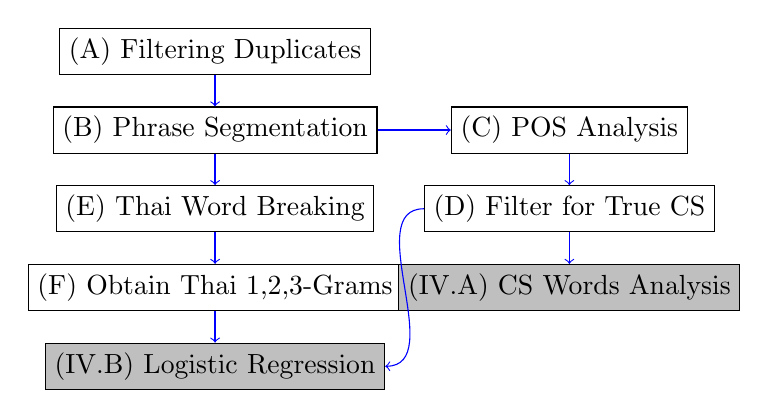
\begin{tikzpicture}
\node[draw] (A) at (0,0) {(A) Filtering Duplicates};
\node[draw] (B) at (0,-1) {(B) Phrase Segmentation};
\node[draw] (E) at (0,-2) {(E) Thai Word Breaking};
\node[draw] (F) at (0,-3) {(F) Obtain Thai 1,2,3-Grams };
\node[draw,fill=lightgray] (J) at (0,-4) {(IV.B) Logistic Regression };
\node[draw] (C) at (4.5,-1) {(C) POS Analysis};
%\node[draw] (C) at (4.5,-1) {(C) Filter Out Punctuations};
\node[draw] (D) at (4.5,-2) {(D) Filter for True CS};
\node[draw,fill=lightgray] (H) at (4.5,-3) {(IV.A) CS Words Analysis};
%\node[draw,fill=lightgray] (J) at (4.5,-4) {(J) Regression Label };

\draw[->,draw=blue] (A) to (B);
\draw[->,draw=blue] (B) to (E);
\draw[->,draw=blue] (E) to (F);
\draw[->,draw=blue] (F) to (J);
\draw[->,draw=blue] (B) to[in=180,out=0] (C);
%\draw[->,draw=blue] (B) to[in=180,out=0] (C);
%\draw[->,draw=blue] (C) to (D);
\draw[->,draw=blue] (D) to (H);
\draw[->,draw=blue] (D) to[in=0,out=180] (J);
%\draw[->,draw=blue] (C) to[in=0,out=0] (D);
\draw[->,draw=blue] (C) to (D);
%\draw[->,draw=blue] (H) to[in=180,out=180] (J);

%\node at (1.0, -1.0) {\textit{a) }};


\end{tikzpicture}
\label{fig:process}
\caption{Data Pre-Processing Steps. The steps in shaded boxes are analyses of results which are explained in Section IV. }
\end{figure}

% (A)
\subsection{Filtering Duplicates}

This phase ensures that there are no duplicate tweets in the data set. The data used are streaming data which contains very little duplicate tweets (same id), however, we find $55$ tweets with duplicate {\tt id\char`_str}  out of $2,583,847$ tweets. 


In addition to obvious duplicates, we filter out retweets. Note that the analysis of code-switching words without filtering retweets out is equivalent to treating a retweet as a regular tweet, which could be justifiable if the non code-switching tweets are as likely to be retweeted as the code-switching tweets. However, this assumption might not hold. Additionally, to perform regression, we need to filter out retweets in order to eliminate the possibility of prediction of seen data in the test set. We filter out tweets that contain the following pattern \verb|r'RT @[\w]+:'| This filter is needed in addition to the {\tt "retweeted":true} tag contained in tweet json format as manual inspection confirms that some tweets that are clearly retweets  have this flag set as {\tt "retweeted":false}. This  can be the case that users manually retweets. The final dataset contains $775,400$ tweets. 

% non empty tweets 756485 (not containing Thai or English words)

% 55

% (B)
\subsection{Phrase Segmentation}
We segmented tweets into a disjoint list of substrings. Each substring either contains only Thai characters (unicode range \verb|[\u0E00-\u0E7F]|) or no Thai character at all. This pre-precessing is needed since the Thai word-breaking library is not meant to break English word  adjacent to Thai word with no space (which occurs quite often in tweet data). The library is also strictly incompatible with input containing unfamiliar unicode, especially ones that represent Emoji or symbols. The thai substrings are processed in (E) to obtain n-grams. The non-Thai strings are processed in (C) for part of speech analysis.



\subsection{Part of Speech Preliminary Analysis}
We define pseudo code-switching instances as the occurrences of English phrases that are adjacent to Thai phrases.  These are not all what we consider   true code-switching instances since words such as `Harry Potter' or `Interstellar' almost, if not always, necessitates the use of the English words. 

The hypothesis is that these pseudo code-switching instances will contain a large number of proper nouns. In addition to proper noun category (denoted by \^{}), we also found marked difference in  part of speech distributions, as shown in Figure~\ref{fig:pos_phrases}. The part of speech  tags are explained with examples in Table~\ref{tab:pos_legend}




\begin{figure}[H]
	\centering
	\includegraphics[clip=true,trim=0 10 0 00,scale=0.45, width=0.4\textwidth]{Results/hist_cs_phrases.png}
	\includegraphics[clip=true,trim=0 10 0 00,scale=0.45, width=0.4\textwidth]{Results/NonCS/distribution_POS_engWords_data_nov17.png}
	\caption{Distribution of Part of Speech for Words in Code Switching Phrases vs Words in English Tweets }
	\label{fig:pos_phrases}
\end{figure}

We use the the observed ratio as an estimate for the probability (which corresponds to the MLE estimate). Figure ~\ref{fig:pos_phrases} shows the sample distribution  for  part of speech  for words that occur in pseudo code-switching English phrases, as well as the part of speech for English words in normal English tweets. There are $201,985$ words that occur in pseudo code-switching phrases. The baseline English tweets contain $822,559$ words. 

%The part of speech 
% distinct????
%The pseudo code-switching phrases contain $201,985$  words. The baseline English tweets contain $82,105$ tweets, consisting of $822,559$ words. 


\begin{table}[h!] 
%~\ref{bib:GimpelEtal}
 \caption{Part of Speech Legend and Examples. See {\tt [1]} for more details.}
\centering % centering table 
\begin{tabular}{c c l c c c rrrrrrr} % creating 10 columns 
\hline\hline % inserting double-line 
POS Tag		&	Tag Meaning	& 	Examples	
\\ [0.5ex] 
\hline 
\verb|N| 	&	common noun & \verb|mv line BTS mama cap winner|	  	 \\ 
\verb|O|  	&	pronoun & 	 \verb|me I Me II US i| 	 \\ 
%\verb|S|  	&	nominal + possessive & 	 0.130297 	 \\ 
\verb|^| 	&	proper noun & 	 \verb|iPhone ELF Facebook  2NE1| 	 \\
%\verb|Z|  	&	proper noun + possessive & 	 0.751134 	 	\\
\verb|L|  	&	nominal + verbal & 	 {\tt ibaekrauhls ID iPhone6Plus}	 \\
%\verb|M|  	&	proper noun + verbal & 	 0.000389 	 \\
\verb|V|  	&	Verb & 	 \verb|vs talk VS read VOTE Rewind| 	 \\
\verb|A|  	&	Adjective & 	 \verb|infinite Favorite Fast|	 \\
\verb|R|  	&	Adverb & 	 \verb|Y forever here alone always| 	 \\
\verb|!|  	&	Interjection & 	 \verb|gt http lt amp IG| 	 \\ 
%\verb|D|  	&	Determiner & 	 (not found) 	 \\ 
\verb|P|  	&	subordinate conjunction & 	 \verb|via by in Like| 	 \\ 
\verb|&|  	&	coordinating conjunction & 	\verb|n and  or But|	 \\ 
\verb|T|  	&	verb particle & 	 \verb|up off down out| 	 \\ 
%\verb|X|  	&	existential & 	 0.022578 	 \\ 
\verb|#|  	&	hashtag & 	 \verb|#codeswitching| 	 \\ 
\verb|@|  	&	at-mention & 	 \verb|@user| 	 \\
\verb|~|  	&	discourse marker & 	 \verb|RT rt Rt PLSRT -rt| 	 \\ 
\verb|U|  	&	URL or email address & 	 \verb|google.com/dtJfg04| 	 \\ 
\verb|E|  	&	emoticon & 	 \verb|x XD T___T T__T -w-| 	 \\ 
\verb|$|  	&	numeral & 	  \verb|2ndWin One 1stWin 10thirty |  	 \\ 
\verb|,|  	&	punctuation & 	 \verb|yg_bear YG_iKONph i5 -v-| 	 \\ 
\verb|G|  	&	other abbreviation & 	 \verb|SM iKON w M PlsRT| 	 \\ 
% [1ex] adds vertical space 32 
\hline % inserts single-line 
\end{tabular} 
\label{tab:pos_legend} 
\end{table} 

In this paper, we will consider the code-switching unigrams as true code-switching as it is generally challenging to determine if the code-switch is true for non unigrams. Figure~\ref{fig:hist_cs_len} shows that we still keep a lot of data by choosing only the unigrams.

\begin{figure}[H]
	\centering
	\includegraphics[clip=true,trim=0 10 0 0,scale=0.45, width=0.4\textwidth]{Results/hist_pseudoCS_len.png}
	\caption{Histogram for number of words in pseudo code-switching phrases. There are $775,345$  pseudo code-switching phrases  contained in  $102,550$ Tweets.}
	\label{fig:hist_cs_len}
\end{figure}

Considering only the (pseudo) code-switching unigrams,  the part of speech distribution is shown in Figure~\ref{fig:pos_uni}.



\begin{figure}[H]
	\centering
	\includegraphics[clip=true,trim=0 10 0 70,scale=0.45, width=0.4\textwidth]{Results/hist_cs_unigrams.png}
	\includegraphics[clip=true,trim=0 10 0 70,scale=0.45, width=0.4\textwidth]{Results/NonCS/distribution_POS_BrownClusterWords.png}
	\caption{Distribution of Part of Speech for Words in Code Switching Unigrams vs Words in English Tweets}
	\label{fig:pos_uni}
\end{figure}




\subsection{Filter for True Code-Switching Words}
From this point on, we will attempt to come up with a filtering rule for true code-switching instances. As mentioned before, we will be considering only code-switching unigrams. 
%turn our attention to code-switching words that are meaningful English words and are not proper nouns. 
In addition, the sample words from tagger ~\ref{tab:pos_legend} also suggest that we keep  only the words with the following part of speech:  \verb| [&,A,O,N,P,R,T,V] | Note that ideally, we should be able to keep a larger set part of speech. However, based on the tags performed on a subsets of twitter words shows in Table ~\ref{tab:pos_legend}, we choose to filter out some potentially meaningful part of speech that ideally we should be able to use such as $L$ (nominal + verbal). 


In addition, there are some proper nouns that passed through the part of speech filter such as {\tt interstellar, divergent, vine, galaxy}. This group contains proper nouns that might be recently popular and consequently is not incorporated in the POS tagger. We manually go through the code-switching words (this is possible due to its relatively small size of distinct words) to identify proper nouns and filter out words in the following list:


\begin{table}[h!] 
 \caption{List of Proper Nouns for Manual Filter}
\centering % centering table 
\begin{tabular}{c c c c c c rrrrrrr} % creating 10 columns 
\hline\hline % inserting double-line 
Proper Noun		&	Explanation		
\\ [0.5ex] 
\hline 
'interstellar' 	&	Movie name	\\
'divergent'		&      Movie name       \\ 
'insurgent'		&      Movie name        \\
'kamikaze'		&      Music band        \\ 
'line'			&      App name       \\
'marvel'		&      Company name        \\
'vine'			&      App name        \\ 
'whiplash'		&      Movie name        \\
'beam'		&    	Singer name          \\
'coke'		&      Company/Product name        \\ 
'muggins'		&      Harry Potter term        \\
'tot'			&      Company name       \\
'galaxy'		&	Product name 	\\
\hline % inserts single-line 
\end{tabular} 
\label{tab:properNouns} 
\end{table} 




% (c)
\subsection{Word Breaking (Thai) }
The Thai phrases in process (B) are the input for word breaking.  For a given Thai phrase or sentence, words are written contiguously without any space between them as seen in example tweets shown in Figure~\ref{fig:ex_csTweets}. %In addition, spaces sometimes are also omitted between English word and Thai words as shown below.   

%???????????????????????????? ???organize??????????????????

%\begin{otherlanguage*}{thai} ?????? event ????? organize ????? ?????????? ????????????????
%\end{otherlanguage*}

%Note: This Tweet has been abridged and modified for demonstration purpose. 

%First, we process tweets by selecting out contiguous Thai characters by regular expression pattern \verb|u'[\u0E00-\u0E7F]+'| which matches Thai characters.
%[????????????????????????????, ???, organize, ??????????????????]

%For each thai phrase that contains only Thai characters, 
We use the library {\tt libthai0.1.4} by Theppitak Karoonboonyanan et al. and a Python interface {\tt PyThai} to break each Thai  phrase into a list of words. The Thai word list will be further processed to obtain n-grams.
%These words are joined back to the original list. 

%For example, the example tweet becomes 
% ??? ?? ?? ?? ?? ??? ????
%[ [??? ??? ?? ???? ??? ???? ???? ??? ??], [???], [organize], [??? ?? ?? ?? ?? ??? ????]]

% (D)
\subsection{Obtaining N-Grams}
%Each word in Thai has its own meaning without being adjacent to other words like in
We choose to obtain 1-,2-,3-grams of the words that have already been broken from process (E). Note that if we were to do n-gram over characters, this should be roughly $1-15$-grams for Thai. Note that due to our pre-processing step (B), we treat any white space, punctuation, and English character in the \emph{original} text as a stopping character for the n-gram sliding window.  %For instance the segmented list  is not included in any $2-$ or $3-$ gram, which should be the case particularly for 
This is appropriate for Thai because a space indicates the end a phrase or a sentence (unlike in English where white spaces indicates the end of a word). Punctuations are also usually not used in the middle of a Thai phrase and therefore their presence are presumed to indicate a switch to a new phrase, if any.

Figure ~\ref{fig:thaingram_logHist} shows the histogram of Thai $1,2,3$-grams obtained from sliding window method on the lists of contiguous Thai words. As regression features, we keep only n-gram that occurs at least $10$ times. This reduces the number distinct n-grams from $3,739,286$ to $119,450$. The total number of n-grams collected is $17,538,739$.

\begin{figure}[H]
	\centering
	\includegraphics[clip=true,trim=0 0 0 0,scale=0.45, width=0.4\textwidth]{Results/ngram_hist_fine.png}
	\caption{Histogram (Log Scale) of Thai 1-,2-,3-grams.}
	\label{fig:thaingram_logHist}
\end{figure}



%That each, we treat each input, e.g., the following three lists %[??? ??? ?? ???? ??? ???? ???? ??? ??], [???], [??? ?? ?? ?? ?? ??? ????]
%as disjoint. 


%For instance, the 2-gram for the  example tweet are 
% [ [??? ???, ??? ??, ?? ????, ???? ???, ??? ????, ????  ????,  ???? ???, ???  ??],
%[], [organize], [??? ??, ?? ??, ?? ??, ?? ??, ?? ???, ???  ????]    ]




%FIGURE of histogram


%Next, we consider the occurrence of  n-grams that occurs at least $10$ times as a feature 

%(E)
%\subsection{Design Matrix and Labels}
%\col{mention sparse}

%Explain regression

%We consider only n-grams that occur at least $10$ times as features and build a sparse matrix of size $NUMTWEET \times NUMDIM$ as a design matrix for regression. 


% (F)
%\subsection{Part of Speech Analysis}





%\subsection{Punctuation Filtering}


%\subsection{CS Labeling}



%Based on the analysis in section (F), we decide to filter out words with part of speech not in the following list.

%TABLE with explanation








%\subsection{CS Words Analysis}



%\subsection{Regression Label}

%\subsection{Code-Switching Prediction}
%We try to be as careful as possible in the process of building the design matrix $X$ to be used for regression. 







%%%%%%%%%%%%%%%%%%%%%%%%%%%%%%%%%%%%%%
%%%%%%%%%%%%%%%%%%%%%%%%%%%%%%%%%%%%%%
%%%%%%%%%%%%%%%%%%%%%%%%%%%%%%%%%%%%%%
%\newpage
\section{Analysis and Results}

\subsection{Analysis of Code-Switching Unigrams}
%From this section on, code-switching will strictly means the occurrence of English word that is not a proper noun and that is adjacent to Thai phrases on either sides. 
%In particular, the filtering process for code-switching words are according to steps (H) described in Section III. 

\begin{figure}[H]
	\centering
	\includegraphics[clip=true,trim=60 10 70 20,scale=0.30, width=0.38\textwidth]{Results/cs_words_filterRT.png}
	\includegraphics[clip=true,trim=50 10 70 20,scale=0.30, width=0.38\textwidth]{Results/cs_words_filterRT_zoom.png}
	\caption{Distribution of part of speech for words in code switching unigrams versus words in English tweets. Dark line shows the line of equal probability. Dashed lines show the lines of probability ratio of $4.0$ and $0.25$.}
	\label{fig:cs_words}
\end{figure}

We are interested in seeing how the code-switching language differs from the normal English language. In particular, we use the twitter data collected from $2008$ to $2012$ containing $56,345,753$ tweets as the baseline English language. This dataset is provided by CMU's Twitter NLP.

% number of distinct words



Figure~\ref{fig:cs_words} shows the words and their associated code-switching probabilities and English tweet probabilities. The probabilities are the observed ratio (or MLE estimate)  given  the group of $2,673$ distinct words that occur in both code-switching and English usage. The total number of code-switching words  are $13,175$ and the total number of English words are $518,410,750$. On average, each word occurs roughly $\frac{13,175}{2,673} \approx 5$ times in code-switching. Figure~\ref{fig:cs_words} show the words that occur in code-switching at least $10$ times. % and has their code-switching probability at least $4$ times or at most $0.25$ times relative to their English probability. The region near 


The words in Figure~\ref{fig:cs_words} might appear to have no apparent structure. There are some words that, for a native speaker, seems to make sense that they are used quite often for code-switching such as party, vote, official, cotton, copy, shop, taxi, sale, mute, etc. Next, we attempt to cluster the code-switching words in order to infer some structural interpretation. 

%Finally, how many CS words, how many distinct. %fig:cs_words





%In addition, since we will be considering the unigrams as only a true code-switching instance, w
\subsubsection{Part of Speech of True Code-Switching Unigrams}
We also consider the distribution of part of speech  but only for  code-switching unigrams after filtering process. The baseline is the English unigrams filtered with the part of speech set \verb| [&,A,O,N,P,R,T,V] |. Figure ~\ref{fig:pos_uni} shows the result. 


\begin{figure}[H]
	\centering
	\subfloat[Distribution of POS for Code-Switching Words\label{fig:test1}]
  {\includegraphics[clip=true,trim=20 10 20 70,width=.45\linewidth]{Results/onlyGoodPOS/cs_unigrams.png}}\hfill
\subfloat[Distribution of POS for English Words\label{fig:test2}]
  {\includegraphics[clip=true,trim=20 10 20 70,width=.45\linewidth]{Results/onlyGoodPOS/eng_brown.png}}\hfill
	\caption{Distribution of Part of Speech for Words in Code Switching Unigrams vs Words in English Tweets}
	\label{fig:pos_uni_goodPOS}
\end{figure}

We note that where there is a somewhat equal balance between noun and verb for normal English usage, there is a disproportionately high number of nouns for code-switching. Adjective, however, is quite on part with verb for code-switching as opposed to normal English usage where adjective is less than half of the verb frequency. This might be because users tend to use words to help describe their feelings (adjective) rather and explain their actions (verb). 


\subsubsection{Brown Clustering}
Next, we attempt to compare the code-switching words with English words using Brown cluster algorithm. The library is obtained from \verb|https://github.com/percyliang/brown-cluster|

Figure~\ref{fig:brown} shows the density of each cluster for words that occur in both code-switching and English tweets. The sample words for each cluster is shown in Table~\ref{tab:sampleBrown}. 

\begin{figure}[H]
	\centering
	\includegraphics[clip=true,trim=0 10 0 70,scale=0.45, width=0.4\textwidth]{Results/brown_cluster10.png}
	\caption{Cluster Density of Code-Switching Words and English Words. Red bars (top) indicates the code-switching densities. Blue bars (bottom) indicate English densities.}
	\label{fig:brown}
\end{figure}


\begin{table}[h!] 
 \caption{Sample Words for Brown Clusters. The words are shown from highest frequency or lowest. }
\centering % centering table 
\begin{tabular}{c c c c c c rrrrrrr} % creating 10 columns 
\hline\hline % inserting double-line 
Cluster		&	Sample Words	
\\ [0.5ex] 
\hline 
0  	&	by, sms, follow,  cc, feeling, live, sus, cotton	 \\ 
1 	&	vs, sexy, you, sale, swag, art, new, social	 \\ 
2  	&	at, tag,  edit, m$\&$m, again, alert, paper, cry 	 \\ 
3 	&	save,  boxset, kitty, user, hashtag, depress, from	 \\
4 	&	vote,  ip, comeback, redcarpet, roommate,  search, sad	\\
5 	&	mama, party, winner, error, inbox, me, beast, only, talk	 \\
6  	&	overdose, empty, read, and, time, kpop, sound, portfolio	 \\
7 	&	mv, sweetie, ep, final, public, local, verb, speed, original 	 \\
8	&	in, me, retro, set, reading, text, begin, dvd, baby, as, story 	 \\
9  	&	w/, mute, cover, ask, via, shop, i, yu, possible, teen, essay 	 \\
% [1ex] adds vertical space 32 
\hline % inserts single-line 
\end{tabular} 
\label{tab:sampleBrown} 
\end{table} 

Note: even though there seem to be density disparities for some clusters such as cluster $5,6,7$, the sample words do not indicate that each cluster is easily interpretable. This might be because the number of clusters used is quite low and therefore words that might be seem to be directly related are forced to be in the same group. The original implementation which performs clustering with $1000$ clusters seem to achieve good results in terms of cluster interpretability. However,  we are quite constrained by the number of code-switching words since there are only $\approx 2000$ distinct words. Figure~\ref{fig:brown100} shows the cluster densities for $100$ clusters. From observation, this is still too few of a cluster number to make the clusters easily interpretable. Sample words for cluster $48$ is [party,  like, official,  support,  morning,  order ] and [baby, sweet,  account, said, country,  1st,  colorful] for cluster $49$. We did not perform statistical test for disparity of cluster densities due to lack of cluster interpretability.



\begin{figure}[H]
	\centering
	\includegraphics[clip=true,trim=0 10 0 70,scale=0.45, width=0.5\textwidth]{Results/brown_cluster100.png}
	\caption{Cluster Density of Code-Switching Words and English Words. Red bars (top) indicates the code-switching densities. Blue bars (bottom) indicate English densities.}
	\label{fig:brown100}
\end{figure}


Note: In addition to brown word clustering, we also attempted a k-medoid cluster based on distance involving path similarity. However, for a large number of words, this algorithm turns out to create disproportionately big/small clusters. The algorithm is also quite slow compared to brown clustering and therefore we did not pursue this approach to the fullest extent. 



%\subsection{Prediction Results}
\subsection{Logistic Regression}
In this section, we are interested in predicting when code-switching occurs in a tweet based on Thai n-grams.  We choose to use logistic regression as a classifier model due to the interpretability each feature's influence (correlation coefficient $\beta$).  Logistic regression is also quite efficient for very high dimensional feature space ( order of magnitude $10^5 - 10^6$) and large data size. 

The target variable for logistic regression is whether code-switching occurs in a tweet. The features are the occurrence of n-gram. The design matrix has $756,485$ number of observations and $119,450$ features. 



\begin{table}[h!] 
 \caption{Average of prediction scores of 5-fold cross validations for both lasso and ridge regression. The predication score is defined by the percentage of correct prediction.}
\centering % centering table 
\begin{tabular}{c c c c c c rrrrrrr} % creating 10 columns 
\hline\hline % inserting double-line 
	Regularization & 	$\lambda$		&	Prediction Score	&	Standard Deviation		%&	Precision	& 	Recall	
\\ [0.5ex] 
\hline 
	Lasso 	& 	$e^{-4}$		&	0.972047 	&	$3.6637 \times 10^{-4}$	\\
	Lasso 	& 	$e^{-3}$		&	0.976628	&
$3.6681 \times 10^{-4}$		\\	
	Lasso 	& 	$e^{-2}$		&	0.980829	&
$3.6053 \times 10^{-4}$           \\	
	Lasso 	& 	$e^{-1}$		&	0.984475	&
$1.5892 \times 10^{-4}$           \\	
	Lasso 	& 	$e^{0}$		&	0.986524	&
$7.2210 \times 10^{-5}$          \\	
	\textbf{Lasso} 	& 	$\mathbf{e^{1}}$		&	\textbf{0.986922}	&
$\mathbf{9.77314 \times 10^{-5}}$          \\	
	Lasso 	& 	$e^{2}$		&	0.986816	&
$2.15595 \times 10^{-5}$           \\	
	Lasso 	& 	$e^{3}$		&	0.986745	&
$3.14490 \times 10^{-5}$           \\	
	Lasso 	& 	$e^{4}$		&	0.986494	&
$7.93141 \times 10^{-6}$           \\	\hline
	Ridge 	& 	$e^{-4}$		&	0.979649	&
$3.08827 \times 10^{-4}$           \\	
	Ridge 	& 	$e^{-3}$		&	0.982186	&
$2.71405 \times 10^{-4}$         \\	
	Ridge 	& 	$e^{-2}$		&	0.984274	&
$1.56487 \times 10^{-4}$           \\	
	Ridge 	& 	$e^{-1}$		&	0.985726	&
$1.23270 \times 10^{-4}$           \\	
	Ridge 	& 	$e^{0}$		&	0.986445	&
$9.32293 \times 10^{-5}$           \\	
	Ridge 	& 	$e^{1}$		&	0.986806	&
$4.93549 \times 10^{-5}$           \\	
	\textbf{Ridge} 	& 	$\mathbf{e^{2}}$		&	\textbf{0.986917}	& 
$\mathbf{4.79543 \times 10^{-5}}$           \\	
	Ridge 	& 	$e^{3}$		&	0.986903	&
$3.95688 \times 10^{-5}$           \\	
	Ridge 	& 	$e^{4}$		&	0.986524	&
$2.18813 \times 10^{-5}$           \\	
% [1ex] adds vertical space 32 
\hline \hline % inserts single-line 
\end{tabular} 
\label{tab:predictionScores} 
\end{table} 

First, we perform a regularized logistic regression with $5$-fold cross-validation to determine the optimal regularization parameter $\lambda$. The penalty term considered are both $\ell_1$ norm (lasso model) and $\ell_2$ norm (ridge regression model) of the coefficient vector $\vec{\beta}$. We use the library {\tt scikitlearn} with the design matrix $X$ in  {\tt Python}'s {\tt scipy} sparse matrix format.

\begin{table}[h!] 
 \caption{Prediction scores for the baseline estimator (predict all non code-switch) and the classifier trained by regularized logistic regression. The scores are based on $20\%$ of data, which contains $151,297$ samples with  $2,098$ code-switching instances. }
\centering % centering table 
\begin{tabular}{c c c c c c rrrrrrr} % creating 10 columns 
\hline\hline % inserting double-line 
Estimator 			&	Accuracy		&	Precision	& 	Recall		&	CS Pred.
\\ [0.5ex] 
\hline 
Flat  						&	 0.98613		& 	 N/A 	&	0.0		& 0.0 	\\ 
Lasso  $\lambda = e^{1}$ 	&	0.98683 		& 	0.7977 	&		0.068		&	178	 \\ 
%Ridge  $\lambda = e^{2}$ 		&	0.98699 		& 	0.8457  	&	0.076	& 188	 \\ 
Lasso  $\lambda = e^{0}$ 	&	 0.987587		& 	0.85484 	&	0.126			&	310	 \\ 
Lasso  $\lambda = e^{-1}$ 	&	 0.990912		& 	0.95471 	&	0.361			&	794	 \\ 
%Ridge  $\lambda = e^{1}$ 		&	0.987515 		& 	0.8828  	&	0.114	& 273	 \\
% [1ex] adds vertical space 32 
\hline % inserts single-line 
\end{tabular} 
\label{tab:scores} 
\end{table} 

The optimal $\lambda$ based on the prediction score for Lasso model ($\lambda = e^1$) leads to a  high-bias estimator that predict predominantly non code-switch. %High $\lambda$ also corresponds to model with lower complexity (less wiggly) that 
If we allow for more variance which corresponds to the assumption that irregularity/code-switching in data are meaningful signals, we obtain a classifier that tends to predict more code-switching as shown for the case $\lambda = e^0, e^{-1}$. %These higher-variance lower-bias predictors predicts more code-switching since the code-switching instances in training date are incorporated as more significant signals.
In the sparse-data situation, we might prefer the high-variance lower-bias predictors since the low-variance one simply needs more data in order to be confident about predicting code-switch. For the Lasso model with $\lambda = e^{-1}$, we obtain the classifier that high relatively high recall of $0.361$ which means that out of all code-switching instances, it can identify $36 \% $ of them. This is reasonably high because given the right features positively correlated to code-switching, the phenomenon occurs with some probability as some users might simply choose to use Thai words instead of code-switching to English. Out of all the identified code-switching, however, $99.09 \% $ are correct. 




Using the Lasso model with $\lambda = e^1$, we perform logistic regression on the entire dataset and analyze the significant features. Out of $119,450$ features, $8,198$ features  are found to be significant at level $\alpha = 0.001$. The number of positive $\beta$ that are significant are $1,918$.


Note: please see analysis for significant Thai n-grams with example tweets in separate Appendix. (due to difficulty of Thai with LaTeX)


%Table ~\ref{tab:predictionScores} shows the optimal parameter {$\lambda = e^1$. } for Lasso regression, based on the percentage of correctness score.  We also analyzes the prediction power of this logistic regression as shown in Table ~\ref{tab:scores}. 












%\subsection{Significant Thai N-Grams}
%Table ~\ref{tab:significantNgram} lists Thai N-grams with positive betas that are significant at level $\alpha = 0.001$.

 

%Next, we demonstrate sample code-switching tweets that contain at least one the significant n-gram with positive beta. 


%%%%%%%%%%%%%%%%%%%%%%%%%%%%%%%%%%%%%%
%%%%%%%%%%%%%%%%%%%%%%%%%%%%%%%%%%%%%%
%%%%%%%%%%%%%%%%%%%%%%%%%%%%%%%%%%%%%%
%\newpage
\section{Conclusion}
We succeed in determining code-switching words at a satisfactory level. From this we build a classifier which is able to predict code-switching instances better than the baseline flat predictor and  analyze significant n-grams that are correlated to code-switching. While there is no immediate interpretation for the significant n-grams, we get a glimpse into what types of n-grams influence code-switching. These types of n-grams tend to be more modern activity such as n-grams with meaning button, apps, concert and some other non-obvious but perhaps more interesting n-grams such as job/event, city, clothes. 



%%%%%%%%%%%%%%%%%%%%%%%%%%%%%%%%%%%%%%
%%%%%%%%%%%%%%%%%%%%%%%%%%%%%%%%%%%%%%
%%%%%%%%%%%%%%%%%%%%%%%%%%%%%%%%%%%%%%
%\newpage
\section{Discussion}
This section discusses the challenges the further improvement that can be made. 
\subsection{Code-Switching Determination}
One of  difficult tasks in this research is the determination of whether a code-switch occurs in given tweet. 
The process employed filters out proper noun  quite well to some extent. However, we find that there are some words that the POS tagger could not have known. An example of this is the following tweet. 


\begin{figure}[H]
	\centering
	\includegraphics[clip=true,trim=0 0 0 0,scale=0.45, width=0.4\textwidth]{Images/CS_Examples/line_cs.png}
	\caption{Example Tweet}
	\label{fig:GS_compare_column_alpha}
\end{figure}

The word {\tt Line} in this case refers to a messaging application that is particularly popular in South East Asia. In this paper, we manually goes through the words and select out the set of words that are most likely proper nouns such as {\tt line, interstellar}, to name but a few. However, it could very well be the case that the tweet actually refers to the word {\tt line} in the usual English meaning.  An improvement for the code-switching determination process would be a classifier that translates the whole phrase into English and performs the tagging. 


\subsection{Sparsity of Code Switching Data}
In this exercise, the  code-switching tweets occurs with frequency roughly $2 \% $. This translates to about $13$K code-switching instances with $2.6$K distinct words. This is quite small compared to the number of words in the English baseline of $800$K distinct words. Given more time and resources, this project can be extended to a larger data set. If we gather enough data such that the number of distinct code-switching words is close to the order of $10-100$K, this will allow for more rigorous analysis on the comparison of code-switching and English word clusters. A natural extension would also be to categorize the words against LIWC. This might also need more code-switching data in order to obtain the significance (if any) as well. 

% An example of a floating figure using the graphicx package.
% Note that \label must occur AFTER (or within) \caption.
% For figures, \caption should occur after the \includegraphics.
% Note that IEEEtran v1.7 and later has special internal code that
% is designed to preserve the operation of \label within \caption
% even when the captionsoff option is in effect. However, because
% of issues like this, it may be the safest practice to put all your
% \label just after \caption rather than within \caption{}.
%
% Reminder: the "draftcls" or "draftclsnofoot", not "draft", class
% option should be used if it is desired that the figures are to be
% displayed while in draft mode.
%
%\begin{figure}[!t]
%\centering
%\includegraphics[width=2.5in]{myfigure}
% where an .eps filename suffix will be assumed under latex, 
% and a .pdf suffix will be assumed for pdflatex; or what has been declared
% via \DeclareGraphicsExtensions.
%\caption{Simulation Results}
%\label{fig_sim}
%\end{figure}

% Note that IEEE typically puts floats only at the top, even when this
% results in a large percentage of a column being occupied by floats.


% An example of a double column floating figure using two subfigures.
% (The subfig.sty package must be loaded for this to work.)
% The subfigure \label commands are set within each subfloat command, the
% \label for the overall figure must come after \caption.
% \hfil must be used as a separator to get equal spacing.
% The subfigure.sty package works much the same way, except \subfigure is
% used instead of \subfloat.
%
%\begin{figure*}[!t]
%\centerline{\subfloat[Case I]\includegraphics[width=2.5in]{subfigcase1}%
%\label{fig_first_case}}
%\hfil
%\subfloat[Case II]{\includegraphics[width=2.5in]{subfigcase2}%
%\label{fig_second_case}}}
%\caption{Simulation results}
%\label{fig_sim}
%\end{figure*}
%
% Note that often IEEE papers with subfigures do not employ subfigure
% captions (using the optional argument to \subfloat), but instead will
% reference/describe all of them (a), (b), etc., within the main caption.


% An example of a floating table. Note that, for IEEE style tables, the 
% \caption command should come BEFORE the table. Table text will default to
% \footnotesize as IEEE normally uses this smaller font for tables.
% The \label must come after \caption as always.
%
%\begin{table}[!t]
%% increase table row spacing, adjust to taste
%\renewcommand{\arraystretch}{1.3}
% if using array.sty, it might be a good idea to tweak the value of
% \extrarowheight as needed to properly center the text within the cells
%\caption{An Example of a Table}
%\label{table_example}
%\centering
%% Some packages, such as MDW tools, offer better commands for making tables
%% than the plain LaTeX2e tabular which is used here.
%\begin{tabular}{|c||c|}
%\hline
%One & Two\\
%\hline
%Three & Four\\
%\hline
%\end{tabular}
%\end{table}


% Note that IEEE does not put floats in the very first column - or typically
% anywhere on the first page for that matter. Also, in-text middle ("here")
% positioning is not used. Most IEEE journals/conferences use top floats
% exclusively. Note that, LaTeX2e, unlike IEEE journals/conferences, places
% footnotes above bottom floats. This can be corrected via the \fnbelowfloat
% command of the stfloats package.







% conference papers do not normally have an appendix

%\newpage
% use section* for acknowledgement
\section*{Acknowledgment}


The author would like to express sincere gratitude for the following NLP-related libraries  that help this project implementation manageable/possible.
\begin{itemize}
\item NLTK
\item Python's langid
\item Python's enchant
\item ark-tweet-nlp-0.3.2
\item ark-CMU Brown cluster implementation 
\item scikitlearn
\end{itemize}





% trigger a \newpage just before the given reference
% number - used to balance the columns on the last page
% adjust value as needed - may need to be readjusted if
% the document is modified later
%\IEEEtriggeratref{8}
% The "triggered" command can be changed if desired:
%\IEEEtriggercmd{\enlargethispage{-5in}}

% references section

% can use a bibliography generated by BibTeX as a .bbl file
% BibTeX documentation can be easily obtained at:
% http://www.ctan.org/tex-archive/biblio/bibtex/contrib/doc/
% The IEEEtran BibTeX style support page is at:
% http://www.michaelshell.org/tex/ieeetran/bibtex/
%\bibliographystyle{IEEEtran}
% argument is your BibTeX string definitions and bibliography database(s)
%\bibliography{IEEEabrv,../bib/paper}
%
% <OR> manually copy in the resultant .bbl file
% set second argument of \begin to the number of references
% (used to reserve space for the reference number labels box)
\begin{thebibliography}{1}

%\bibitem{IEEEhowto:kopka}
%H.~Kopka and P.~W. Daly, \emph{A Guide to \LaTeX}, 3rd~ed.\hskip 1em plus
%  0.5em minus 0.4em\relax Harlow, England: Addison-Wesley, 1999.


\bibitem{bib:GimpelEtal}
K. Gimple, N. Schneider, B. O'Conner et at., \emph{Part-of-Speech Tagger for Twitter: Annotation, Features, and Experiments}

\bibitem{bib:BrownCluster}
P. Liang. \emph{Semi-Supervised Learning for Natural Language}, Department of Electrical Engineering and Computer Science, MIT, 2005.
\verb|https://github.com/percyliang/brown-cluster|

%\bibitem{bib:wordClusterNiceInterpretation}
%\verb|http://www.ark.cs.cmu.edu/TweetNLP/cluster_viewer.html| shows $1000$ word clusters by Brown algorithms. 



\end{thebibliography}




\end{document}


%%%%%%%%% FIGURE
\begin{figure}[H]
	\centering
	\includegraphics[clip=true,trim=0 10 0 70,scale=0.45, width=0.4\textwidth]{../../Results/GS/comparison14_LN_decliningRate.png}
	\caption{Average Best Cost over 5 Trials for Column-Wise Neighborhood for Different Parameter $\alpha_i,\alpha_f$}
	\label{fig:GS_compare_column_alpha}
\end{figure}



%%%%%%%%% Table

\begin{table}[h!] 
 \caption{Average Delta Cost over $100$ Neighbors for Various Neighborhood Definitions} % title name of the table 
\centering % centering table 
\begin{tabular}{c c c c c c rrrrrrr} % creating 10 columns 
\hline\hline % inserting double-line 
Neighborhood Option &   $\alpha$ & Average Delta Cost    %& RMSE with User Mean  & Numter of Iterations &  $\gamma$ &\multicolumn{7}{c}{Sum of Extracted Bits} 
\\ [0.5ex] 
\hline % inserts single-line 
 
% Entering 1st row 
 %& &soft &1 & $-1$ & 1 & 1 & $-1$ & $-1$ & 1 \\[-1ex] 
%\raisebox{1.5ex}{Police} & \raisebox{1.5ex}{5}&hard 
%& 2 & $-4$ & 4 & 4 & $-2$ & $-4$ & 4 \\[1ex] 
Column-wise Constant $\alpha$  	&	1.0 & 	 0.025499 	 \\ 
Column-wise Constant $\alpha$  	&	2.0 & 	 0.062459 	 \\ 
Column-wise Constant $\alpha$  	&	4.0 & 	 0.130297 	 \\ 
Column-wise Constant $\alpha$  	&	8.0 & 	 0.302554 	 \\
Column-wise Constant $\alpha$  	&	16.0 & 	 0.751134 	 	\\
Column-wise Constant $\alpha$  	&	32.0 & 	 2.415786 	 \\
Element-wise Constant $\alpha$  	&	1.0 & 	 0.000389 	 \\
Element-wise Constant $\alpha$  	&	2.0 & 	 0.001880 	 \\
Element-wise Constant $\alpha$  	&	4.0 & 	 0.006716 	 \\
Element-wise Constant $\alpha$  	&	8.0 & 	 0.003288 	 \\
Element-wise Constant $\alpha$  	&	16.0 & 	 0.006320 	 \\
Element-wise Constant $\alpha$  	&	32.0 & 	 0.022578 	 \\
% [1ex] adds vertical space 32
\hline % inserts single-line 
\end{tabular} 
\label{tab:SA_aveDeltaCost} 
\end{table} 

